\documentclass{beamer}
\title[Practical Application 2]
	{Practical Application 2}
\subtitle{Machine Learning}
\author[Cerezo Pomykol, Jan]
	{Jan Cerezo Pomykol\newline
	\href{mailto:j.cerezo@alumnos.upm.es}{\small\texttt{j.cerezo@alumnos.upm.es}}}

\institute[Universidad Politécnica de Madrid]
	{Universidad Politécnica de Madrid\newline
	 ETSIINF}
\date{November 22, 2022}

\usetheme{Warsaw}
\usecolortheme{lily}

\setbeamertemplate{navigation symbols}{}

\addtobeamertemplate{navigation symbols}{}{%
    \usebeamerfont{footline}%
    \usebeamercolor[fg]{footline}%
    \hspace{1em}%
    \insertframenumber/\inserttotalframenumber
}

\begin{document}

\maketitle

\begin{frame}
\frametitle{Problem Description}
\begin{columns}
\begin{column}{0.5\textwidth}
Dry Bean Dataset:
\begin{itemize}
\item 13611 instances
\item 16 variables
\item 7 classes
\item \href{https://archive.ics.uci.edu/ml/datasets/Dry+Bean+Dataset\#}{\small\color{blue}Source}
\end{itemize}
\centering
\raisebox{-2cm}{
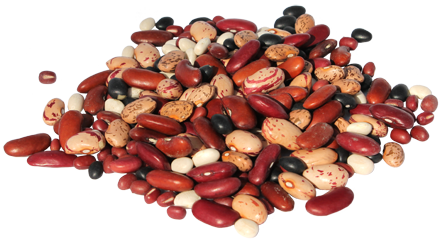
\includegraphics[width=0.7\textwidth]{beans}
}
\end{column}
\begin{column}{0.25\textwidth}
\begin{tiny}
\begin{itemize}
\item[-] Area
\item[-] Perimeter
\item[-] Major axis length
\item[-] Minor axis length
\item[-] Aspect ratio
\item[-] Eccentricity
\item[-] Convex area
\item[-] Equivalent diameter
\item[-] Extent
\item[-] Solidity
\item[-] Roundness
\item[-] Compactness
\item[-] ShapeFactor1
\item[-] ShapeFactor2
\item[-] ShapeFactor3
\item[-] ShapeFactor4
\end{itemize}
\end{tiny}
\end{column}

\begin{column}{0.25\textwidth}
\begin{scriptsize}
\begin{itemize}
\item[-] Seker
\item[-] Barbunya
\item[-] Bombay
\item[-] Cali
\item[-] Dermosan
\item[-] Horoz
\item[-] Sira
\end{itemize}
\end{scriptsize}
\end{column}
\end{columns}
\end{frame}

\begin{frame}
\frametitle{Methodology}
\begin{columns}
\begin{column}{0.5\textwidth}
\begin{itemize}
\item Software: \textbf{Weka}
\item Classification algorithms:
\begin{tiny}
\begin{itemize}
	\scriptsize
	\item Logistic Regression
	\item Naive Bayes
	\item Tree Augmented Naive Bayes
	\item Linear Discriminant Analysis
	\item Fusion
	\item Stacking
	\item Bagging
	\item Random Forest
	\item Boosting
	\item Naive Bayes Tree
	\item Logistic Model Tress
\end{itemize}
\end{tiny}
\item Feature Subset Selection
\begin{itemize}
	\scriptsize
	\item No FSS
	\item Univariant Filter
	\item Multivariant Filter
	\item Wrapper Approach
\end{itemize}
\end{itemize}
\end{column}

\begin{column}{0.5\textwidth}
\centering
\resizebox{\textwidth}{!}{
\begin{tabular}{||l|l||}
	\hline
	Algorithm & Weka Function\\
	\hline
	Logistic Regression & functions.Logistic\\
	Naive Bayes & bayes.NaiveBayes\\
	Tree Augmented Naive Bayes & bayes.BayesNet\\
	Linear Discriminant Analysis & functions.LDA\\
	Fusion & meta.Vote \\
	Stacking & meta.Stacking\\
	Bagging & meta.Bagging\\
	Random Forest & trees.RandomForest\\
	Boosting & meta.AdaBoostM1\\
	Naive Bayes Tree & trees.NBTree\\
	Logistic Model Trees & trees.LMT\\
	\hline
\end{tabular}
}
\newline\newline
\resizebox{\textwidth}{!}{
\begin{tabular}{||l|l||}
	\hline
	FSS algorithm & Weka Function\\
	\hline
	No FSS & -\\
	Univariant Filter & attributeSelection.InfoGainAttributeEval\\
	Multivariant Filter & attributeSelection.CfsSubsetEval\\
	Wrapper Approach & attributeSelection.WrapperSubsetEval\\
	\hline
\end{tabular}
}
\end{column}
\end{columns}
\end{frame}

\begin{frame}
\frametitle{Results}
\framesubtitle{Selected Attributes}
\centering
\resizebox{0.8\textwidth}{!}{
\begin{tabular}{||l|c|c|c|c|c|c|c|c|c|c|c|c|c|c||}
	\hline
	Attribute &
	\rotatebox[origin=c]{90}{No FSS} &
	\rotatebox[origin=c]{90}{Univariant} &
	\rotatebox[origin=c]{90}{Multivariant} &
	\rotatebox[origin=c]{90}{Wrapper (Logistic)} &
	\rotatebox[origin=c]{90}{Wrapper (Naive Bayes)} &
	\rotatebox[origin=c]{90}{Wrapper (TAN)} &
	\rotatebox[origin=c]{90}{Wrapper (LDA)} &
	\rotatebox[origin=c]{90}{Wrapper (Fusion)} &
	\rotatebox[origin=c]{90}{Wrapper (Stacking)} &
	\rotatebox[origin=c]{90}{Wrapper (Bagging)} &
	\rotatebox[origin=c]{90}{Wrapper (Random Forest)} &
	\rotatebox[origin=c]{90}{Wrapper (Boosting)} &
	\rotatebox[origin=c]{90}{Wrapper (NBTree)} &
	\rotatebox[origin=c]{90}{Wrapper (LMT)}\\
	\hline
	Area &  & $\bullet$ & & & & & $\bullet$ & & & $\bullet$ & $\bullet$ & $\bullet$ & & $\bullet$\\
    Perimeter & $\bullet$ & $\bullet$ & $\bullet$ & $\bullet$ & $\bullet$ & $\bullet$ & $\bullet$ & $\bullet$ & $\bullet$ & $\bullet$ & & $\bullet$ & $\bullet$ & $\bullet$\\
    MajorAxisLength & $\bullet$ & $\bullet$ & $\bullet$ & $\bullet$ & & & & & $\bullet$ & & $\bullet$ & & & $\bullet$\\
    MinorAxisLength & $\bullet$ & $\bullet$ & $\bullet$ & $\bullet$ & & $\bullet$ & & $\bullet$ & & & & & $\bullet$ & \\
    AspectRatio & $\bullet$ & & $\bullet$ & & & $\bullet$ & & & $\bullet$ & & & & & \\
    Eccentricity & $\bullet$ & & & & & & & & $\bullet$ & & & & & \\
    ConvexArea & $\bullet$ & $\bullet$ & $\bullet$ & $\bullet$ & & & $\bullet$ & & $\bullet$ & & & & & $\bullet$\\
    EquivDiameter & $\bullet$ & $\bullet$ & & $\bullet$ & & & & & $\bullet$ & & & & & $\bullet$\\
    Extent & $\bullet$ & & $\bullet$ & $\bullet$ & & $\bullet$ & $\bullet$ & $\bullet$ & $\bullet$ & $\bullet$ & $\bullet$ & $\bullet$ & & \\
    Solidity & $\bullet$ & & & $\bullet$ & & & & $\bullet$ & & $\bullet$ & $\bullet$ & & $\bullet$ & $\bullet$\\
    Roundness & $\bullet$ & & $\bullet$ & $\bullet$ & $\bullet$ & $\bullet$ & & $\bullet$ & $\bullet$ & $\bullet$ & $\bullet$ & & $\bullet$ & $\bullet$\\
    Compactness & $\bullet$ & & $\bullet$ & & $\bullet$ & $\bullet$ & $\bullet$ & $\bullet$ & & $\bullet$ & $\bullet$ & & $\bullet$ & \\
    ShapeFactor1 & $\bullet$ & $\bullet$ & $\bullet$ & $\bullet$ & $\bullet$ & $\bullet$ & & & & $\bullet$ & $\bullet$ & & & \\
    ShapeFactor2 & $\bullet$ & $\bullet$ & $\bullet$ & $\bullet$ & & & & & $\bullet$ & $\bullet$ & & & & $\bullet$\\
    ShapeFactor3 & $\bullet$ & & & & & & & & & & $\bullet$ & $\bullet$ & & \\
	ShapeFactor4 & $\bullet$ & & $\bullet$ & $\bullet$ & $\bullet$ & $\bullet$ & $\bullet$ & $\bullet$ & $\bullet$ & $\bullet$ & $\bullet$ & & $\bullet$ & $\bullet$\\
    \hline
    \textbf{N attributes} & 16 & 8 & 11 & 11 & 5 & 8 & 6 & 7 & 10 & 9 & 9 & 4 & 6 & 9\\
    \hline
\end{tabular}
}
\end{frame}

\begin{frame}
\frametitle{Results}
\framesubtitle{Classifier scores}
\centering
\resizebox{0.95\textwidth}{!}{
\begin{tabular}{||l|l|l|l|l|l|l|l|l|l|l|l||}
	\hline
	Dataset &
	\rotatebox[origin=c]{90}{Logistic} &
	\rotatebox[origin=c]{90}{Naive Bayes} &
	\rotatebox[origin=c]{90}{TAN} &
	\rotatebox[origin=c]{90}{LDA} &
	\rotatebox[origin=c]{90}{Fusion} &
	\rotatebox[origin=c]{90}{Stacking} &
	\rotatebox[origin=c]{90}{Bagging} &
	\rotatebox[origin=c]{90}{Random Forest} &
	\rotatebox[origin=c]{90}{Boosting} &
	\rotatebox[origin=c]{90}{NBTree} &
	\rotatebox[origin=c]{90}{LMT}\\
	\hline
	Original & 92.60 & 89.71 & 91.47 & 90.18 & 91.26 & 91.28 & 89.72 & 92.52 & 89.71 & 89.57 & 92.49\\
	Uni. Filter & 92.14 & 84.09 & 89.90 & 89.22 & 90.00 & 90.29 & 84.03 & 91.04 & 84.09 & 87.67 & 91.94\\
	Mult. Filter & 92.57 & 90.20 & 91.24 & 90.05 & 91.58 & 91.74 & 90.31 & 92.47 & 90.20 & 90.63 & 92.41\\
	Wr. (Logistic) & 92.70 & 89.01 & 91.47 & 90.03 & 91.47 & 91.53 & 89.08 & 92.53 & 89.01 & 89.66 & 89.01\\
	Wr. (N. Bayes) & 92.09 & 91.23 & 91.54 & 89.84 & 89.01 & 91.77 & 91.21 & 92.16 & 91.23 & 91.55 & 92.16\\
	Wr. (TAN) & 92.36 & 90.76 & 91.60 & 89.83 & 91.72 & 91.62 & 90.80 & 92.33 & 90.76 & 90.69 & 92.27\\
	Wr. (LDA) & 92.30 & 88.23 & 90.42 & 91.17 & 91.35 & 91.56 & 88.34 & 91.74 & 88.23 & 89.57 & 92.35\\
	Wr. (Fusion) & 92.39 & 91.05 & 91.29 & 90.58 & 91.91 & 91.24 & 91.05 & 92.68 & 91.05 & 90.88 & 92.44\\
	Wr. (Stacking) & 92.55 & 89.42 & 91.66 & 89.86 & 91.38 & 92.20 & 89.45 & 92.46 & 89.42 & 89.97 & 92.41\\
	Wr. (Bagging) & 92.53 & 90.77 & 91.44 & 89.45 & 91.58 & 91.78 & 90.75 & 92.70 & 90.77 & 90.90 & 92.54\\
	Wr. (R. Forest) & 92.38 & 90.66 & 91.27 & 89.72 & 91.58 & 91.53 & 90.65 & 92.84 & 90.66 & 90.33 & 92.56\\
	Wr. (Boosting) & 91.12 & 80.83 & 89.60 & 88.85 & 89.39 & 89.69 & 80.89 & 91.11 & 80.83 & 89.48 & 91.42\\
	Wr. (NBTree) & 92.21 & 91.22 & 91.24 & 90.56 & 91.89 & 91.17 & 91.22 & 92.46 & 91.22 & 91.27 & 92.27\\
	Wr. (LMT) & 92.45 & 84.75 & 91.02 & 90.32 & 91.22 & 91.30 & 84.80 & 92.28 & 84.75 & 89.82 & 92.52\\
    \hline 
\end{tabular}
}
\end{frame}

\begin{frame}
\frametitle{Results}
\framesubtitle{Training time}
\centering
\resizebox{0.95\textwidth}{!}{
\begin{tabular}{||l|l|l|l|l|l|l|l|l|l|l|l||}
	\hline
	Dataset &
	\rotatebox[origin=c]{90}{Logistic} &
	\rotatebox[origin=c]{90}{Naive Bayes} &
	\rotatebox[origin=c]{90}{TAN} &
	\rotatebox[origin=c]{90}{LDA} &
	\rotatebox[origin=c]{90}{Fusion} &
	\rotatebox[origin=c]{90}{Stacking} &
	\rotatebox[origin=c]{90}{Bagging} &
	\rotatebox[origin=c]{90}{Random Forest} &
	\rotatebox[origin=c]{90}{Boosting} &
	\rotatebox[origin=c]{90}{NBTree} &
	\rotatebox[origin=c]{90}{LMT}\\
	\hline 
	Original & 57.5 & 0.02 & 0.14 & 0.02 & 0.17 & 1.67 & 0.19 & 3.99 & 1.17 & 11.51 & 14.38\\
	Uni. Filter & 2.39 & 0.01 & 0.06 & 0.01 & 0.07 & 0.7 & 0.09 & 3.1 & 0.61 & 5.83 & 10.58\\
	Mult. Filter & 3.89 & 0.01 & 0.09 & 0.01 & 0.11 & 1.06 & 0.15 & 3.18 & 0.84 & 7.17 & 11.41\\
	Wr. (Logistic) & 5.81 & 0.01 & 0.09 & 0.01 & 0.11 & 1.06 & 0.13 & 3.21 & 1.14 & 10.54 & 12.27\\
	Wr. (N. Bayes) & 1.37 & 0.01 & 0.03 & 0.01 & 0.04 & 0.45 & 0.08 & 2.38 & 0.46 & 1.92 & 8.39\\
	Wr. (TAN) & 2.18 & 0.01 & 0.06 & 0.01 & 0.07 & 0.74 & 0.1 & 3.14 & 0.51 & 6.52 & 9.58\\
	Wr. (LDA) & 1.99 & 0.01 & 0.04 & 0.01 & 0.07 & 0.53 & 0.08 & 2.48 & 0.39 & 2.9 & 13\\
	Wr. (Fusion) & 1.97 & 0.01 & 0.05 & 0.01 & 0.06 & 0.63 & 0.09 & 2.46 & 0.58 & 5.23 & 9.86\\
	Wr. (Stacking) & 2.69 & 0.01 & 0.07 & 0.01 & 0.09 & 0.92 & 0.12 & 3.21 & 0.99 & 8.71 & 10.74\\
	Wr. (Bagging) & 2.44 & 0.01 & 0.07 & 0.01 & 0.09 & 0.82 & 0.12 & 3.17 & 0.67 & 5.63 & 10.57\\
	Wr. (R. Forest) & 2.51 & 0.01 & 0.07 & 0.01 & 0.09 & 0.82 & 0.11 & 3.21 & 0.87 & 8.61 & 10.33\\
	Wr. (Boosting) & 0.97 & 0.01 & 0.03 & 0.01 & 0.03 & 0.36 & 0.06 & 2.18 & 0.46 & 1.43 & 8.26\\
	Wr. (NBTree) & 0.96 & 0.01 & 0.04 & 0.01 & 0.06 & 0.53 & 0.09 & 2.44 & 0.45 & 3.96 & 9.05\\
	Wr. (LMT) & 7.95 & 0.01 & 0.06 & 0.01 & 0.08 & 0.83 & 0.11 & 3.28 & 0.56 & 8.26 & 16.41\\
    \hline 
\end{tabular}
}
\end{frame}

\begin{frame}
\frametitle{Results}
\framesubtitle{Logistic Regression}
\centering
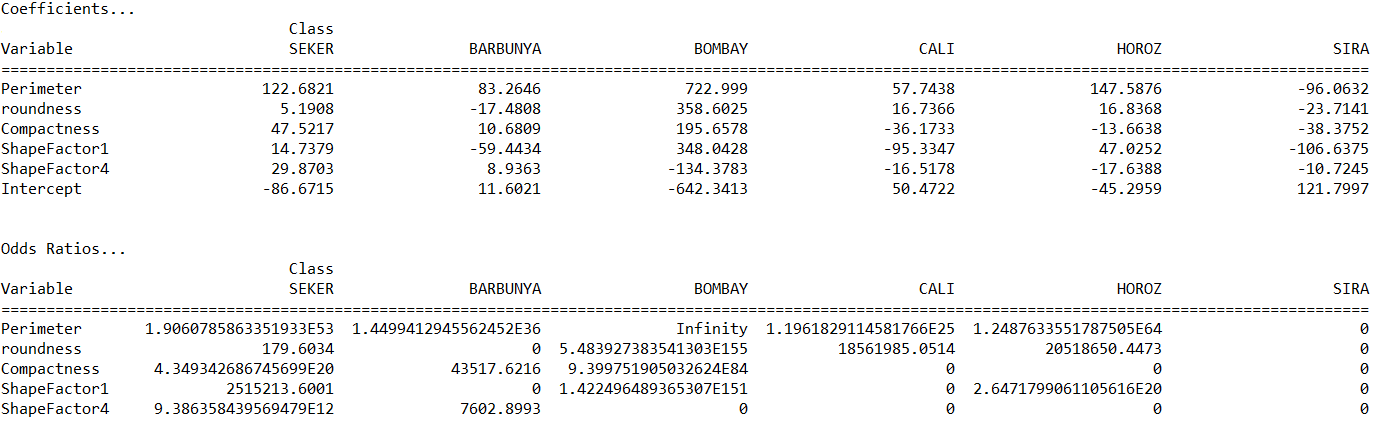
\includegraphics[width=\textwidth]{logistic}
\end{frame}

\begin{frame}
\frametitle{Results}
\framesubtitle{Naive Bayes}
\centering
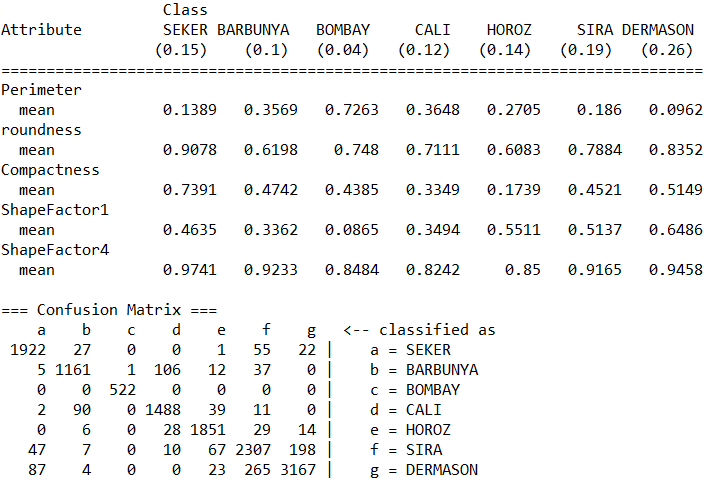
\includegraphics[width=\textwidth]{naivebayes}
\end{frame}

\begin{frame}
\frametitle{Results}
\framesubtitle{Tree Augmented Naive Bayes}
\centering
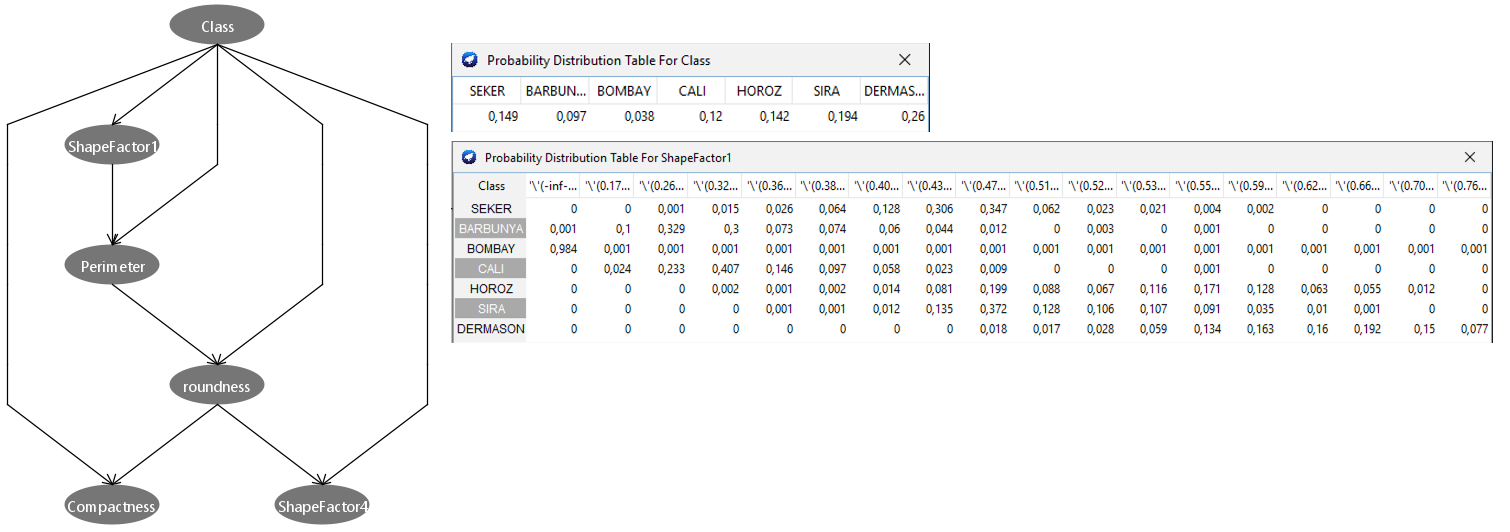
\includegraphics[width=\textwidth]{TAN}
\end{frame}

\maketitle

\end{document}
